\documentclass{standalone}
\usepackage{graphicx}	
\usepackage{amssymb, amsmath}
\usepackage{color}

\usepackage{tikz}
\usetikzlibrary{calc, arrows.meta}
\usepackage{pgfmath}

\definecolor{light}{RGB}{220, 188, 188}
\definecolor{mid}{RGB}{185, 124, 124}
\definecolor{dark}{RGB}{143, 39, 39}
\definecolor{highlight}{RGB}{180, 31, 180}
\definecolor{gray10}{gray}{0.1}
\definecolor{gray20}{gray}{0.2}
\definecolor{gray30}{gray}{0.3}
\definecolor{gray40}{gray}{0.4}
\definecolor{gray60}{gray}{0.6}
\definecolor{gray70}{gray}{0.7}
\definecolor{gray80}{gray}{0.8}
\definecolor{gray90}{gray}{0.9}
\definecolor{gray95}{gray}{0.95}

\newcommand*{\offset}{0.025}

\begin{document}

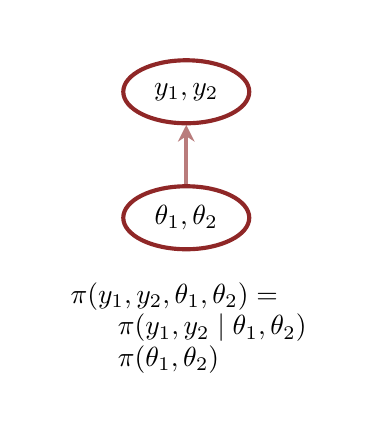
\begin{tikzpicture}[scale=0.2, thick]

  \draw[white] (-10, -16) rectangle (10, 8);

  \pgfmathsetmacro{\r}{2}

  \coordinate (A) at (0, -4);
  \coordinate (B) at (0, +4);

  \draw[-{Stealth[length=6pt, width=6pt]}, shorten >=12, color=mid, line width=1.5] (A) -- (B);
  
  \node[anchor=west] at (-8, -9) { $\pi(y_{1}, y_{2}, \theta_{1}, \theta_{2}) = $ };
  \node[anchor=west] at (-5, -11) { $\pi(y_{1}, y_{2} \mid \theta_{1}, \theta_{2})$ };
  \node[anchor=west] at (-5, -13) { $\pi(\theta_{1}, \theta_{2})$ };

  \filldraw[fill=white, draw=dark, line width=1.5] (A) circle [x radius={2 * \r}, y radius={\r}]
  node[color=black] { $\theta_{1}, \theta_{2}$ };
    
  \filldraw[fill=white, draw=dark, line width=1.5] (B) circle [x radius={2 * \r}, y radius={\r}]
  node[color=black] { $y_{1}, y_{2}$ };

\end{tikzpicture}

\end{document}  